\documentclass{sig-alternate}
\newtheorem{theorem}{Theorem}
\newtheorem{lemma}{Lemma}
\newtheorem{definition}{Definition}
\newtheorem{corollary}{Corollary}
\usepackage{algorithm}
\usepackage{algorithmic}
\usepackage{graphicx}
\usepackage{multirow}
\usepackage{subfigure}
\pdfpagewidth=8.5in
\pdfpageheight=11in
\usepackage[small,it]{caption}
\newcommand{\squishlist}{
 \begin{list}{$\bullet$}
  { \setlength{\itemsep}{0pt}
     \setlength{\parsep}{3pt}
     \setlength{\topsep}{3pt}
     \setlength{\partopsep}{0pt}
     \setlength{\leftmargin}{1.5em}
     \setlength{\labelwidth}{1em}
     \setlength{\labelsep}{0.5em} } }

\newcommand{\squishlisttwo}{
 \begin{list}{$\bullet$}
  { \setlength{\itemsep}{0pt}
     \setlength{\parsep}{0pt}
    \setlength{\topsep}{0pt}
    \setlength{\partopsep}{0pt}
    \setlength{\leftmargin}{2em}
    \setlength{\labelwidth}{1.5em}
    \setlength{\labelsep}{0.5em} } }

\newcommand{\squishend}{
  \end{list}  }
    
\setlength{\abovecaptionskip}{0pt}
\setlength{\belowcaptionskip}{0pt} 

\begin{document}

\title{CrowdBuzz: Trend Discovery and Evolution in \\Social Messaging Systems}

\numberofauthors{2} 
\author{
\alignauthor Krishna Y. Kamath\\
       \affaddr{Texas A\&M University}\\
       \affaddr{College Station, TX 77843}\\
       \email{kykamath@cs.tamu.edu}
\alignauthor James Caverlee\\
       \affaddr{Texas A\&M University}\\
       \affaddr{College Station, TX 77843}\\
       \email{caverlee@cse.tamu.edu}
}

\maketitle
\begin{abstract}
In this paper, we study the problem of automatically discovering and tracking the evolution of \textit{group-based trends} in highly-dynamic social messaging systems like Twitter and Facebook. Unlike trend-tracking systems that aggregate individual actions or posts (e.g., counting tweets including the phrase ``super bowl''), we are interested to track the conversational communication-based patterns across groups of users. These ad-hoc ``crowds'' of users provide an opportunity to identify emergent crowd-based topics of interest that reflect the natural conversational nature of social messaging systems. Two of the salient features of the proposed approach are (i) an efficient locality-based clustering approach for identifying crowds of users in near real-time compared to more heavyweight static clustering algorithms; and (ii) a crowd tracking and evolution approach for linking crowds across time periods. We find that the locality-based clustering approach results in empirically high-quality clusters relative to static graph clustering techniques at a
fraction of the computational cost. Based on a three month snapshot of Twitter consisting of
 711,612 users and 61.3 million messages, we show how the proposed approach can
identify and track interesting crowds based on the Twitter communication structure and find crowd-based topics of interest.

%At its core, CrowdBuzz relies on two key components: (i) an online graph clustering component for identifying important crowds at a particular time based on messages sent between users; and (ii) a crowd tracking and evolution component for linking crowds across time periods. One of the novel contributions of CrowdBuzz is its online social graph clustering approach that is inspired by the Min-Cut graph clustering algorithm for static graphs. 
% and topics that generate high crowd interest (but little individual interest),
% and topics that generate high individual interest (but little crowd interest).
\end{abstract}


\section{Introduction}
\label{sec:introduction}
With the rise of large-scale online social networks, there has been a growing
interest in mining these networks for information discovery, brand management
(e.g., what are users saying about the new iPhone), and other data mining
applications \cite{guo:pattern, zheleva:affiliation, cha:filkr, matsuo:gravity}.
The past few years have seen the development of a number of successful
tools for aggregating online \textit{buzz} (e.g., BlogPulse
\cite{website.blogpulse}, BlogScope \cite{bansal:blogscope}, Meme-tracker
\cite{leskovec:meme}).
% Similarly, Facebook
% has deployed the Lexicon tool for aggregating the posts of users in their social
% network, to reveal how many users are posting about particular topics and give
% insight into the general mood of the network.  
In a related direction, Google
Trends aggregates individual user search queries to provide important insights
into rising or falling issues (e.g., health care, queries like ``coupon'' that
may help predict the direction of the economy \cite{choi:google}), comparison of
subjects (e.g., ipod versus zune, federer versus nadal). These trend discovery
tools are even showing promise for public health and disaster recovery efforts
(e.g., Google Flu Trends).

%In most of these example systems, buzz is a function of the aggregated actions of many individuals, e.g., by counting the number of people searching for ``zune'' or the number of Facebook members posting about ``ipods''. This type of trend analysis is fundamentally \textit{user-centric} by tracking the aggregate of posts from many individuals. 

In many trending systems, a given term $t$ is often tracked over the aggregate of many individual actions or posts, e.g., by counting the number of people searching for ``zune'' or the number of Facebook members posting about ``ipods''. However, these systems may overlook \textit{conversations} occurring between participants that are related to the topic but don't necessarily include the actual term being trended over. In addition, the conversational buzz associated with users actually communicating with each other directly about a topic may be a strong indicator of an emergent online phenomenon worth identifying. Discovering these conversational groupings (what we call \textit{crowds}) can support crowd-based trending topics in addition to the more traditional individual-based trending topics.  %The topics can be given their own weight, just as in the user-centric model, based on several factors of the crowd. 



%talking to each other may 

%``crowd'' is a strong indicator of an emergent online phenomenon that may be worth identifying and directing to interested users.




%This type of trend analysis is fundamentally \textit{user-centric}. With the inherent social-based connectivity in social media, we are interested to examine the communication patterns between users and how these communication patterns may support a \textit{group-centric} notion of buzz. Fundamentally, the group-centric approach, shown in Figure~\ref{fig:single-multi}, seeks to capture the organic buzz that occurs when groups of people talk amongst themselves.
% ; in contrast the
% user-centric approach is typically a one-sided affair, capturing user monologues
% and not necessarily the natural back-and-forth of natural communication among
% users participating in a group.

%Our fundamental insight is that ``crowd''-based emergent information holds the key to effective personalized dissemination of interesting and relevant real-time web information. A single user action -- for example, posting a picture of a smoke plume to Flickr -- though perhaps interesting itself, does not convey a strong community or social-based importance to the user action. In contrast, a flurry of activity associated with a ``crowd'' is a strong indicator of an emergent online phenomenon that may be worth identifying and directing to interested users. Identifying coherent crowds in real-time across a potentially vast collection of non-obviously connected user actions is a major challenge.

But how do we identify \textit{conversations} in the first place? Historically, direct communication between people has been mostly unobservable or
unavailable for analysis by large-scale aggregation services. For example,
private email and instant messages between two users are typically not made
available for natural reasons. But with the rise of new social messaging systems
like Twitter and Facebook, communications between users can be monitored. For example, Twitter
supports the public messaging of users through the inclusion of $@\langle username \rangle$
in a Twitter post (a ``tweet''). So a tweet from the user \textit{nod} can be
addressed to the user \textit{kykamath} like so: ``@kykamath What do you think
about the new iPod?''. This type of observable communication is on the rise and a
significant portion of all messages posted on Twitter, with estimates placing the
percent of all tweets containing the $@\langle username \rangle$  at 30\% (or about 7 million
observable communications per day) \cite{website.gigatweet}. Similar messaging
functionality has recently been adopted by Facebook.

Given these observable communication patterns, we are interested to explore whether we can identify ad-hoc crowds of
users that reflect the real-time interests and affiliations of users? Unlike the
more static and perhaps staler group-based membership offered on many social
networks (e.g., member of Texas A\&M community), this type of 
% , fan of college football),
communication-based crowd discovery promises organic and highly-temporal group
interest identification. 
% Compared to traditional social mining approaches which
% aggregate individual user keywords, by discovering crowds of users based on their
% interactions, we may discover organic linkages among the users. 
% Similarly,
% crowd-based buzzworthy topics may indicate a depth of interest in a subject that
% is not reflected in the straightforward aggregation of user keywords in
% undirected public pronouncements (e.g., status updates, blog
% posts).
However identifying crowds is challenging. Social messaging systems like Twitter
and Facebook have potentially 100s of millions of communicating users inserting
new messages into the system at a high-rate. Even if we can identify a crowd at a
point-in-time, we must additionally track the crowd over time as users join,
multiple crowds merge, and as crowds disband. To deliver up-to-date  crowd
information to group-based trending tools and social mining analytics, the discovery and evolution
approaches must support efficient and near real-time execution.

With these opportunities and challenges in mind, we study the problem of automatically discovering and tracking the evolution of \textit{group-based trends} in highly-dynamic social messaging systems like Twitter and Facebook. Concretely, we propose an efficient locality-based clustering approach for identifying crowds of users in near real-time compared to more heavyweight static clustering algorithms. This locality-based approach relies on the spatial and temporal locality evident in systems like Twitter. Additionally, we propose a crowd tracking and evolution approach for linking crowds across time periods according to varying degrees of evolution granularity (e.g., for tracking very bursty crowds that grow and disperse over several hours versus longer-lived crowds that may last for weeks). Based on a one-week snapshot of Twitter consisting of 706,000 users and 20.3 million messages, we find that the locality-based clustering approach results in empirically high-quality clusters relative to static graph clustering techniques at a fraction of the computational cost. We also  illustrate how the proposed approach can identify and track interesting crowds based on the Twitter communication structure and find crowd-based topics of interest.


% CrowdBuzz relies on two key components: (i) a dynamic graph clustering component for identifying important crowds at a  particular time based on messages sent between users; and (ii) a crowd tracking and evolution component for linking crowds across time periods.  One of the novel  contributions of CrowdBuzz is its dynamic social graph clustering approach that is inspired by the Min-Cut graph clustering algorithm for static graphs. We find  that the dynamic graph clustering component results in empirically high-quality  clusters relative to static graph clustering techniques at a fraction of the  computational cost. Based on a one-week snapshot of Twitter consisting of 250,000  users and 1.2 million messages, we show how CrowdBuzz can identify interesting  crowds based on the Twitter communication structure, topics that generate high  crowd interest (but little individual interest), and topics that generate high  individual interest (but little crowd interest).


%In this paper, we study the problem of automatically discovering and tracking the evolution of \textit{group-based trends} in highly-dynamic social messaging systems like Twitter and Facebook. Unlike trend-tracking systems that aggregate individual actions or posts (e.g., counting tweets including the phrase ``super bowl''), we are interested to track the conversational communication-based patterns across groups of users. These ad-hoc ``crowds'' of users provide an opportunity to identify emergent crowd-based topics of interest that reflect the natural conversational nature of social messaging systems. Two of the salient features of the proposed approach are (i) an efficient locality-based clustering approach for identifying crowds of users in near real-time compared to more heavyweight static clustering algorithms; and (ii) a crowd tracking and evolution approach for linking crowds across time periods. We find that the locality-based clustering approach results in empirically high-quality clusters relative to static graph clustering techniques at a fraction of the computational cost. Based on a one-week snapshot of Twitter consisting of 706,000 users and 20.3 million messages, we show how the proposed approach can identify and track interesting crowds based on the Twitter communication structure and find crowd-based topics of interest.


%At its core, CrowdBuzz relies on two key components: (i) a dynamic graph clustering component for identifying important crowds at a particular time based on messages sent between users; and (ii) a crowd tracking and evolution component for linking crowds across time periods. One of the novel contributions of CrowdBuzz is its dynamic social graph clustering approach that is inspired by the Min-Cut graph clustering algorithm for static graphs. We find that the dynamic graph clustering component results in empirically high-quality clusters relative to static graph clustering techniques at a fraction of the computational cost. Based on a one-week snapshot of Twitter consisting of 250,000 users and 1.2 million messages, we show how CrowdBuzz can identify interesting crowds based on the Twitter communication structure, topics that generate high crowd interest (but little individual interest), and topics that generate high individual interest (but little crowd interest).

% (i) a dynamic graph clustering component for identifying important crowds at a
% particular time; (ii) a crowd tracking and evolution component for linking
% clusters across time periods; and (iii) a crowd visualization and analytics
% component

\begin{figure}[!t]
\begin{center}
\includegraphics[width=3.5in]{../../images/cikm2010/intro}
\caption{Example of crowd discovery in twitter. The table shows the
interactions of users at different time intervals and the corresponding crowds
discovered.}
\label{fig:intro-example}
\end{center}
\end{figure}

\subsection{Crowd Discovery Example}
An example of crowd discovery based on communication between users is shown in
Figure. \ref{fig:intro-example}. The second column in the table shows the
twitter messages sent between users and the third column shows the communication
graph for the interval. To keep the example simple we use the number of
messages transmitted between users as edge weights in the communication
graph and reduce the weight by 1 if no messages are sent in a particular time
interval. The weight is reduced to remove stale users from a crowd. The actual
algorithm in the paper uses a more complex edge weight scheme. The last
column shows the corresponding crowds discovered. In our algorithm we use
graph clustering to identify crowds. But, to simplify this example we use graph
connectivity to identify crowds.

In the first time interval 2 messages are exchanged between A-B and C-D. The
communication graph obtained is shown in the third column. The interaction
between users results in creation of 2 crowds as shown. In the next interval A
and C communicate with each other. This results in the 2 crowds merging
together to form a single crowd. In a real crowd users who do not get
involved in the discussion get bored and move away from the crowd. In the
$3^{rd}$ interval, we observe that user D who has not interacted with rest of
the users for sometime is removed from the crowd and froms a singleton. Finally in
the $5^{th}$ interval user C, like D before, breaks from the crowd and form a
singleton. Thus based on the user communication we can determine user crowds.


\section{Twitter Dataset}
To study crowd detection in a real-world setting, we focus on the Twitter
microblogging service. Through a mix of crawling and API calls to the Twitter
service, we collected a sample of tweets from October $1^{st}$ to December
$31^{st}$, 2008, accounting for 2208 hours (see Table~\ref{table:dataset} for
details). The dataset includes over 710,000 users and over 61.3 million status
updates (``tweets'') of 140 characters or less. Users can annotate their tweets
via the inclusion of hashtags (e.g., ``\#redsox'') to indicate a particular
topic. Similarly, users can include \textit{@mentions} of the form $@\langle
username \rangle$ within a tweet to reference another user. While these
\textit{@mentions} can serve many purposes, the most popular use is as a simple
messaging framework, so that a message posted by user $u_1$ including @$\langle
u_2 \rangle$ is considered a message from $u_1$ to $u_2$.
% (note that users other than $u_2$ may view this public message as well).

\begin{table}[h]
\centering
\label{table:dataset}
\begin{tabular}{|l|r|r|}
\hline
\textbf{Property} & \textbf{Total} & \textbf{Per hour avg.} \\ \hline
Users & 711,612 & 18,713 \\ \hline
Total tweets & 61,314,203 & 27,769 \\ \hline
Messages (@$<u>$) & 20,394,030 & 9,236\\ \hline
User pairs & 3,756,619 & 9,310\\ \hline
% Average degree & 3.48 & - \\ \hline
\end{tabular}
\caption{Twitter dataset properties.}
\end{table}

Of the, 61.3 million tweets in the dataset, 20.4 million contain the $@\langle
username \rangle$ syntax and are considered messages from one user to another.
3.7 million pairs of users are connected by these messages. The hourly
distribution of tweeting users, user pairs, and messages sent is shown in
Figure~\ref{fig:data-distribution}. All are strongly correlated, following a
clear daily and weekly patterns.

\begin{figure}[!t]
\begin{center}
\includegraphics[width=3.5in]{../../images/cikm2010/userInteractions}
\caption{Oct 1 - Dec 31, 2008: Number of users, the number of pairs of users
who have at least one message between them, and the number of messages sent.}
\label{fig:data-distribution}
\end{center}
\end{figure}

%In addition, we observe that messages on Twitter display strong temporal and spatial locality. By \textit{temporal locality}, we mean that messages  BLAH BLAH BLAHB. By \textit{spatial locality}, we mean that messages in the BLAH BLABH ALBHA LBHABH ALBHALBHA BLHA. BLAH BLABH ALBH ABLH ALBHA.  Approximately 1\% of nodes impacted 


\section{Problem Statement}
Given the large and growing size of social messaging systems like Twitter and Facebook,  we are interested to explore group formation in these systems and how this group formation can impact the detection of online trends.  Users may be grouped along a number of dimensions including content-based, geographic-based, communication-based, and so on. We focus on the challenge of uncovering and tracking groups of users -- what we refer to as \textit{crowds} -- according to their communication patterns. Intuitively, a crowd is a time-sensitive collection of users who have messaged each other within some recent window of time. Based on the communication patterns, we hope to identify organic \textit{conversations} occurring between participants for identifying trends.

%are related to the topic but don't necessarily include the actual term being trended over. 


%In many trending systems, a given term $t$ is often tracked over the aggregate of many individual actions or posts, e.g., by counting the number of people searching for ``zune'' or the number of Facebook members posting about ``ipods''. However, these systems may overlook \textit{conversations} occurring between participants that are related to the topic but don't necessarily include the actual term being trended over.  Our system is group-centric in that we seek to discover crowds based on conversation patterns, and then from that crowd, we derive trending topics.  


%\squishlist
%\item \textit{Interest-based grouping}: Reflecting groups of users who share a common interest, e.g., users posting messages about a presidential debate.
%\item \textit{Geographic-based grouping}: Reflecting groups of users who are geographically bounded, e.g., users posting messages from Dallas, Texas.
%\item \textit{Communication-based grouping}: Reflecting groups of users who are actively messaging each other, e.g., users coordinating a meeting.
%\squishend



Formally, we view the users and their communications with other users in a social messaging
system as a \textit{time-evolving communication network}. Let $G(V,E)$ be an
undirected graph with $|V| = n$ vertices and $|E| = m$ edges, where each vertex
corresponds to a user in the social messaging system and an edge corresponds to a
communication between two users. The weight of an edge between vertices $u$ and
$v$ is represented by $w(u, v)$. Each edge is associated with the time of the last communication between two users: $EdgeTime(u,v)$.  Additionally, we will view the graph $G$ as the adjacency list $A$, where $A(u, v) = w(u, v)$ if $(u, v)$ exists, else $A(u, v) = 0$.

Viewing a social messaging system like Twitter as a time-evolving communication network, we face two key challenges:


%Communication patterns These crowds of users are intended to reflect 

%can be further refined by \textit{interest-based grouping} 
%Users may be grouped along a number of dimensions, including (but not limited to):

%\squishlist
%\item \textit{Interest-based grouping}: Reflecting groups of users who share a common interest, e.g., users posting messages about a presidential debate.
%\item \textit{Geographic-based grouping}: Reflecting groups of users who are geographically bounded, e.g., users posting messages from Dallas, Texas.
%\item \textit{Communication-based grouping}: Reflecting groups of users who are actively messaging each other, e.g., users coordinating a meeting.
%\squishend
%By considering the content similarity of user tweets via standard information retrieval techniques or by probabilistic topic models (e.g., LDA \cite{}), users can be grouped according to their interests -- e.g., sports, bLAH, Blah. 


\textbf{Challenge \#1: Crowd Discovery.}  The first challenge is to identify a set of crowds at any moment in time. Social messaging systems like Facebook and Twitter are extremely large (on the order of 100s of millions of unique users), placing huge demands on the computational cost of traditional community detection approaches (which can be $O(n^3)$ in the number of users). And since these services are characterized by a
high-rate of messages, the discovered crowds may become stale quickly, resulting in the need to re-identify crowds (again, incurring the high cost of community detection).


\textbf{Challenge \#2: Crowd Evolution.} In addition to identifying crowds at any moment in time, the second challenge is to track the evolution of crowds across time. For example, as groups of users begin communicating about an upcoming event (say the Super Bowl), the evolution approach should can track the users participating in this crowd and give
insights into the crowd dynamics leading up to and after the event. Since crowds may evolve at different rates, we must be careful in tracking bursty crowds that grow and disperse over several hours versus longer-lived crowds that may last for weeks.

%However, the bursty nature of user communication places demands on crowd evolution to accurately track these highly-temporal based clusters.

%Evolution module can analyze the discovered crowds from the previous module at system-specified time intervals to provide varying degrees of evolution granularity (e.g., for tracking very bursty crowds that grow and disperse over several hours versus longer-lived crowds that may last for weeks).


%dynamic clustering \cite{saha:clustering,gorke:clustering}, etc. 

%In the context of real-time crowd discovery in social messaging systems, however, these graph clustering approaches face challenges. 




%he groups of users discussing the event, until a peak during the event, and finally the ...


%The function of this module is to build a hierarchy of clusters called cluster hierarchy graph. This module accepts a set of clusters $K_s$ at time $t_s$ from the clustering module and for every cluster $C_c$ in $K_s$ it then determines its parent cluster $C_p$ in $K_{s-1}$, if it exists. It then adds an edge between the two clusters $C_c$ and $C_p$. The algorithm to build a hierarchy graph is given in Section~\ref{sub-sec:hierarchy-graph}.

%\subsection{Approach:}
%crowd discovery
%crowd evolution




%Output of this module is the current set of clusters maintained by the clustering algorithm. It sends this out to the next module at regular intervals.

% ... This is the central module in our architecture. We will be using an online
% clustering algorithm in this module. Online and offline algorithms expect same
% input to be give in different formats. An offline algorithm requires entire
% input to be available before start of the algorithm, while an online algorithm
% can process input as it arrives piece-by-piece. Since our application doesn't
% have entire input initially, we use an online algorithm. The  motivation and
% details of this algorithm are given in Section~\ref{sec:graph-clustering}.

% The online clustering algorithm continuously maintains a set of clusters for
% the current set of vertices. Any time an edge is added, the algorithm updates
% the set of clusters accordingly. The clustering module takes a tuple $(u_1,
% u_2, m)$ as input. Since, we will be using graph theoretic approach to
% clustering, it maps every user $u$ to a vertex $v$ and the tuple to an edge
% $e$.  The module then uses {\scshape AddEdge}$(v_1, v_2, w)$ procedure to pass
% the newly added edge $e$ to the online clustering algorithm. The procedure
% {\scshape AddEdge}$(v_1, v_2, w)$ is described in the
% Section~\ref{sec:graph-clustering}.

% Output of this module is the current set of clusters maintained by the
% clustering algorithm. It sends this out to the next module at regular
% intervals. This is shown in Figure~\ref{fig:architecture}, where output from
% clustering module is sent to the hierarchy generator module at regular
% intervals $t_1, t_2, t_3 \ldots t_s$.


%\cite{saha:clustering,THAT NEW DYNAMIC CLUSTERING PAPER}

\section{Crowd Discovery and Evolution}
\label{sec:crowd-discovery}
In an effort to tackle these challenges, we propose an efficient locality-based
crowd discovery and evolution approach. We view crowd discovery as a form of
\textit{clustering in time-evolving communication networks}. Formally, a crowd
$C$ is a set of vertices and $K$ is the set of all crowds in $G$. $C_i$
represents the $i^{th}$ crowd in $K$. Vertices are assigned to one and only one
crowd, i.e., $ C_i \cap C_j = \phi, \forall C_i, C_j \in K$. To identify crowds,
we can directly use of many existing approaches, including spectral clustering
\cite{dhillon:multilevel}, min-cut clustering \cite{flake:cut-clustering}, among
many others. In practice, however, these and related graph clustering approaches
can be $O(n^3)$ in the number of nodes (users in our case), which is unreasonable
considering the large size of Twitter and the needs of trend-based applications
to identify crowds in near real-time. To overcome these issues, we rely on two
key insights:

\squishlist

\item  First, the addition of a new edge to the time-evolving communication network $G$ (i.e., a new message from one user to another at time $t$) should only impact a small number of crowds and not the entire graph. We have confirmed this \textit{spatial locality} on Twitter: for each new message observed in our dataset (corresponding to an edge insertion in the communication network), we find that only about 1\% of users are within two hops, meaning that an edge insertion has only a local effect. Hence, we can leverage this spatial locality of impact to reduce the cost of updating all crowds in the network. 

\item Second, messages in the social messaging system should impact the time-evolving communication network based on their recency, with older messages having less impact on the discovered crowds than do more recent messages. We refer to this emphasis on the present as \textit{temporal locality} to indicate the degree to which past messages can influence the current state of crowds.

\squishend



%In the following ...


%that edge weights should reflect temporal locality (e.g., decaying based on communication recency).  the strength of association between two users in a social messaging system may depend on the recency of their communication (e.g., a message from $u_1$ to $u_2$ today should be considered a stronger signal of their common crowd membership than a message from $u_1$ to a third user $u_3$ a month ago), meaning that a crowd discovery approach based on graph clustering should carefully consider how to decay edge weights

%Third, the strength of association between two users in a social messaging system may depend on the recency of their communication (e.g., a message from $u_1$ to $u_2$ today should be considered a stronger signal of their common crowd membership than a message from $u_1$ to a third user $u_3$ a month ago), meaning that a crowd discovery approach based on graph clustering should carefully consider how to decay edge weights. Fourth, the bursty nature of user communication demands a crowd discovery approach that can capture these highly-temporal based clusters.





%In this section we present the approach to discover user crowds. We first
%show an example of crowd discovery and then formally describe the problem and
%the algorithms used to discover crowds.





%[NEW] Based on these observations, we propose a new class of highly-efficient locality-based clustering algorithms. Locality-based clustering is developed on the notions that (i) changes in a small region of a graph should not affect the entire graph;  and (ii) that edge weights should reflect temporal and interest locality (e.g., decaying based on communication recency). 


%Compared to min-cut clustering \cite{flake:cut-clustering} and related approaches (with $O(n^3)$ time complexity), this locality-based approach can result in $O(k^3)$ complexity, where $k$ is the largest crowd size in $K$. 





%Similarly, every crowd $C$ is associated with the time of last communication of any of its users $ClusterTime(C)$ 

% \begin{itemize}



% \end{itemize}

% In the following three sections, we present these three BLAH BLA HBALHB.

%Recently, there has been some work examining dynamic graph clustering with provable quality guarantees \cite{saha:clustering,THAT NEW DYNAMIC CLUSTERING PAPER}.


%Time-evolving communication networks are huge with large number of vertices. In these graphs, a small change, for example, modification of an edge in one part of a graph should not affect the entire graph. Applying the same intuition in context of clustering, we can say that modification of an edge between two clusters or within a cluster should not affect the rest of the clusters. By handling these modifications locally, we can prevent the need to touch the entire graph, and hence make the clustering algorithm more efficient. We apply this intuition to develop our algorithm.

%Our algorithm has two parts. The first part handles clustering of the graph and second handles reading of clusters. 

%\begin{itemize}
%\item \textbf{Phase 1:} All clusters in the graph are kept independent and hence changes in a particular cluster doesn't effect the other clusters. The first part of the algorithm is applied when an edge is added to the graph. We identify the clusters that get effected by addition of this edge and take action to ensure cluster quality specified in Section~\ref{sub-sec:quality} is maintained. 
%\item \textbf{Phase 2:} The second part of the algorithm is applied when an application tries to read the clusters. We need to handle this part separately because weights of edges change with time and there might be a time lag between when the clusters were created (updated) and when they are read.
%\end{itemize}

%In the next section we describe algorithm to handle edge addition and then present an ideal algorithm to read clusters. We then give two efficient approximations of the ideal algorithm.

\subsection{Locality-Based Graph Clustering}
We propose a locality-based graph clustering approach that is designed to leverage both the temporal and spatial locality observed in Twitter and similar social messaging systems. The general principles can be applied across different graph clustering techniques. For concreteness in this paper, we shall focus on a locality-based version of the traditional min-cut clustering algorithm. 

\subsubsection{Min-Cut Clustering}
First, we present some preliminaries to describe min-cut clustering, before introducing our locality-based enhancements. Intuitively, min-cut clustering identifies clusters with more intra-cluster edges than inter-cluster edges.

\medskip
\noindent\textbf{Minimum cut:} The minimum cut of $G$ with respect to vertices
$s$ and $t$, where $s \in S, t \in T$, is defined as partition of $V$ into $S$
and $T$ such that, the total weight of edges connecting the partitions is
minimum. This is represented as $c(S, T)$. For an undirected graph $G$ we can
define a weighted tree $T_G$ called the minimum-cut tree \cite{hu:mincut}. We can
determine $c(S, T)$ by finding the path from $s$ to $t$ in $T_G$, where the value
of $c(S, T)$ is equal to the sum of the weights of edges on this path.

\medskip
\noindent\textbf{Min-cut clustering:} The min-cut clustering algorithm
\cite{flake:cut-clustering} clusters a graph $G$ first by adding an artificial
sink $t$. All of the vertices of $G$ are connected to the artificial sink with an
edge capacity of $\alpha$, to form a modified graph $G'$, where $\alpha$ is a
parameter guiding the quality guarantees of the resulting clusters. The
minimum-cut tree $T'$ for $G'$ is then calculated. The connected components of
$T'$ obtained after removing the artificial sink $t$ are clusters in $G$.


% \algsetup{indent=2em}
% \newcommand{\CutClustering}{\ensuremath{\mbox{\sc CutClustering}}}
% \begin{algorithm}
% \caption{$\CutClustering(G(V,E), \alpha)$}\label{alg:cut-clustering}
% \begin{algorithmic}
% \STATE $V' = V \cup t$
% \FORALL{$v \in V'$}
% \STATE Connect $t$ to $v$ with a capacity of $\alpha$
% \ENDFOR
% \STATE $G'(V', E')$ be the graph obtained from $G$
% \STATE Calculate the minimum-cut tree $T'$ for $G'$
% \STATE Remove $t$ from $G'$
% \RETURN All connected components of $G'$ 
% \end{algorithmic}
% \end{algorithm}



%\textbf{Expansion:} The expansion of the (sub)graph, $\Psi(S)$, is the minimum expansion over all the cuts of the (sub)graph. The expansion of clusters in $G$ is defined as the minimum expansion over all the clusters. The larger the value of expansion, the better is the clustering algorithm.

% The quality of clusters generated using the min-cut clustering algorithm is
% closely related to the quality requirements. Following
% \cite{flake:cut-clustering}, we base the cluster quality on the expansion of a
% cut  $(S, \bar{S})$ in $G$

%\begin{align*}
% \label{expansion}
%\Psi(S) &= {\frac{\sum_{u \in S, v \in \bar{S}}w(u,v)}{min\{|S|,|\bar{S}|\}}} = {\frac{c(S, \bar{S})}{min\{|S|,|\bar{S}|\}}}
%\end{align*}

 %The expansion of the (sub)graph is the minimum expansion over all the cuts of
 %the (sub)graph. The expansion of clusters in G is minimum expansion over all
 %the clusters. The larger the value of expansion, the better is the clustering algorithm.

\medskip
Min-cut clustering relies on a special parameter $\alpha$ to
ensure the quality of the clusters generated, where:

% $\alpha$ provides a lower bound on intra-cluster expansion and an upper bound on inter-cluster expansion. Given $S \subset V$ and $P, Q \subset S | P \cap Q = \phi, P \cup Q = S$, $\alpha$ is defined as:
\begin{align}
\label{eq:clustering-quality}
\frac{c(S, V-S)}{|V-S|} \leq \alpha \leq \frac{c(P, Q)}{min(|P|, |Q|)}
\end{align} 

By tuning this $\alpha$ parameter, the number and size of the resulting clusters can be varied (from one large cluster with all nodes to a trivial clustering consisting of $n$ singleton nodes).


\subsubsection{Exploiting Temporal Locality}
To reflect the temporal locality observed on Twitter, the first component of our crowd discovery algorithm is an edge impact damping
factor for reducing the weight of older edges. This is important so that the
crowds discovered reflect fresh (and more impactful) messages in the system.
Recall that each edge in the time-evolving communication network is associated
with an edge weight $w(u, v)$ and the time of the last communication between the
two users: $EdgeTime(u,v)$. We can modulate the weight $w(u, v)$ to reflect the
application semantics -- for example, by considering edge weights for all $u$ and
$v$ as $w(u, v) = 1$, we can treat all edges the same (regardless of when the
messages between users were sent -- meaning that crowds discovered at time $t$ reflect the entire history of communication in the network). Another possibility is to consider only edges
within a fixed time-window: e.g., $w(u, v) = 1$ for all edges with $EdgeTime(u,v)
- CurrentTime > \beta$, where $CurrentTime$ ($CT$) is the current time in the
system and $\beta$ is some windowing parameter. In this case, messages sent more
than $\beta$ time units earlier are completely disregarded by the crowd discovery
system, resulting in crowds that reflect the up-to-the-minute state of the network.

Intuitively, since messages sent more recently reflect the current interests of
users in the social messaging system, we propose an edge impact damping function
that gradually fades the impact of older messages relative to newer ones.
Concretely, we propose an exponentially decaying impact factor based on a damping
coefficient  $\xi$ for controlling the rate of damping. For edges $(u, v) |
w(u,v) > 0 $ we  update the new edge weight $w^*(u, v)$ using this exponential fading as:

\[
w^*(u, v) = w(u, v)- \log(CT - EdgeTime(u, v))\times \xi
\]

%$DampEdge:(w(u, v), EdgeTime(u,v), CurrentTime, \xi) \rightarrow w(u, v)$.
% \begin{align*}
% For\ w(u,v) = 1:\\
% DampEdge(u, v) =
% &w(u, v) - w(u, v) \times\ \xi\ \times\\
% &\log(CT - ET(u,v))\\
% For\ w(u,v) > 1:\\
% DampEdge(u, v) =
% &w(u, v) - \log(w(u, v)) \times\ \xi\ \times\\
% &\log(CT - ET(u,v))
% \end{align*}



%To have a notion of time in our algorithm let $CurrentTime$ ($CT$) be a pointer to current time in the system. The function $Time(C)$ gives the time when cluster $C$ was last updated and $EdgeTime(u,v)$ ($ET$) gives the time when the edge $(u, v)$ was last updated. 



\begin{figure}[!t]
\begin{center}
\includegraphics[width=3.5in]{../../images/www/edgeDecay}
\caption{The graphs show changes to edge weights when $DampEdge(u, v)$ is
applied. The above graph shows actual edge weight and the bottom graphs show
effect of damping the edges.}
\label{fig:edge-decay}
\end{center}
\end{figure}


To illustrate the impact of this exponential fading, a typical communication graph between two users is shown in Figure~\ref{fig:edge-decay}.
The upper plot shows number of messages (actual weight) exchanged between two users
and the bottom plots shows the damped edge weights. The middle plot shows the effect of damping with $\xi = 0.3$ and
the bottom plot with $\xi = 1.0$. The value of $\xi$ determines the type of
crowd we identify. Crowds forming slowly can be identified with lower values
of $\xi$ while higher value of $\xi$ identifies crowds forming quickly.
Hence, this parameter can be tuned according to the particular application requirements. 

Note that the overall clustering algorithm will occasionally need to damp the edges of all nodes in a cluster. We show in Algorithm~\ref{alg1}, the straightforward adaptation of the single edge damping to the damping of all nodes in a cluster $C$.

\algsetup{indent=2em}
\newcommand{\DampCluster}{\ensuremath{\mbox{\sc DampCluster}}}
\begin{algorithm}
\caption{$\DampCluster(C)$}\label{alg:cluster-damp}
\begin{algorithmic}
\STATE \textbf{Update Edges:} Update the edge weights in the
adjacency matrix for all internal and cut edges $(u,v)$ in $C$.
\begin{center}
$A(u, v) = A(u, v)- \log(CT - EdgeTime(u, v))\times \xi$
\end{center}
\end{algorithmic}
\label{alg1}
\end{algorithm}


% between the users results in the weight between the two users reduced overtime. Our algorithm handles formation and breaking of communities based on the weight obtained from $DampEdge$.

\subsubsection{Exploiting Spatial Locality}
Given the edge impact factor, we next consider how the spatial locality of communication on Twitter can enable efficient locality-based clustering. Recall that locality-based clustering is developed on the notion that changes in
 a small region of a graph should not affect the entire graph. Hence, on
 insertion of a new edge (corresponding to a new message between users in the social
 messaging service), we can apply the locality-based clustering to a small number of
 affected crowds only and not the entire set of crowds. This helps in saving the
 computational expense of clustering the entire graph.  Since
 this approximation does not have the strong quality guarantees of min-cut
 clustering, we empirically validate the clustering quality
in Section~\ref{sec:experiments}.

As a first step, we present a local version (see Algorithm~\ref{alg:cluster-recluster}) of the standard min-cut clustering algorithm that can be applied to a particular subgraph of $G$. Given a set of local crowds $S$ to re-cluster, the algorithm first contracts $G$ to $G'$. It then creates a new graph $G''$ by adding an artificial sink $t$ to $G'$ and connecting all the vertices of $S$ to $t$ with edges of capacity $\alpha$ and all the vertices in $(V'-S)$ with edges of capacity of $\alpha|V-S|$. It then determines the minimum-cut tree $T''$ for $G''$. The connected components obtained after removing $t$ from $T''$ are the new crowds. In this way, only a small portion of the communication network is impacted, leading to more efficient clustering that re-clustering the entire network.


\algsetup{indent=2em}
\newcommand{\LocalCutClustering}{\ensuremath{\mbox{\sc LocalCutClustering}}}
\begin{algorithm}
\caption{$\LocalCutClustering(S)$}\label{alg:cluster-recluster}
\begin{algorithmic}
\STATE \textbf{1. Contract $G$:} Reduce $G$ to  $G'$ by replacing
vertices $V-S$ with a new vertex $x$. All the resulting loops are deleted and parallel
edges are replaced with a single edge with weight equal to the sum of the
edges.% \cite{flake:cut-clustering}. 
\STATE \textbf{2. Expand $G'$:} Construct a new graph $G''$ by
adding vertex $t$ to $G'(V', E')$. Connect $t$ to $v, \forall v \in S$ with
edge capacity of $\alpha$ and $t$ to $v', \forall v' \in (V'-S)$ with edge
capacity of $\alpha|V-S|$.% \cite{flake:cut-clustering}\cite{saha:clustering}.
\STATE \textbf{3. Minimum-cut tree:} Determine minimum-cut tree
$T''$ for $G''$. The connected components obtained in $T''$ after removing vertices $t$ and $x$ from it are
the clusters in $S$. 
\end{algorithmic}
\label{alg2}
\end{algorithm}




%Locality-Based clustering essentially has 2 phases. (i) A clustering phase during which local crowds are clustered without affecting the entire graph and, (ii) An edge insertion phase during which we determine the crowds that are affected by the insertion and check if these crowds need to be re-clustered.

%We first present some  preliminary definitions followed by the locality-cut clustering algorithm. We end the section by giving the time complexity of the algorithm.

% [[NEED TO MAKE SURE ALL OF OUR NOTATIONS ARE CORRECT AND CONSISTENT; ALSO NEED TO MAKE SURE WE ARE CONSISTENT IN OUR USE OF CROWD / CLUSTER AND THESE NEW SUBSECTIONS -- e.g., LOCAL CROWD DETECTION, LOCALITY-BASED, etc.]]
%\subsubsection{Locality-Based Clustering: Overview}%

% where $\alpha$ is a lower bound on intra-cluster expansion and an upper bound
% on inter-cluster expansion. %The details of determining $\alpha$ are given in \cite{flake:cut-clustering}.


%Second, the addition of a new edge to the time-evolving communication network $G$ (i.e., a new message from one user to another at time $t$) should only impact a small number of crowds and not the entire clustering. Hence, we can leverage this locality of impact to reduce the cost of updating all clusters in the network.

The question remains, though -- which crowds should be selected for the local version of cut clustering described in Algorithm~\ref{alg2}? Selecting too many crowds for re-clustering may result in expensive computation, whereas selecting too few crowds may result in poor crowd quality. We adopt an approach on each edge insertion that  that makes use of temporal and spatial locality to discover crowds in a time evolving communication network. The psuedocode for the algorithm is given in Algorithm~\ref{alg:add-edge}.


%We now present the algorithm that makes use of temporal and spatial locality to discover crowds in a time evolving communication network. The algorithm is an iterative algorithm that is executed on every edge addition. 


\algsetup{indent=2em}
\newcommand{\AddEdge}{\ensuremath{\mbox{\sc UpdateClustersOnEdgeInsertion}}}
\begin{algorithm}[!ht]
\caption{$\AddEdge(u,v,w)$}\label{alg:add-edge}
\begin{algorithmic}
\STATE \textbf{1. Initialization:} If the edge added has vertices
that have not been observed before add them to vertex set $V$. Create singleton clusters
for the new vertices %with  their $ClusterTime$ value set to $CurrentTime$ 
and add them to cluster set $K$. 
\STATE \textbf{2. Update the adjacency matrix: }\\
\begin{center}
$A(u,v) = A(u,v) + w$
\end{center}
\STATE \textbf{3. Clustering:} Let $u$, $v$ belong to clusters $C_u$ and $C_v$
respectively. Update the edge weights within the clusters using DampCluster()
function defined before. Now depending on the conditions that match perform the
corresponding clustering operations: 
\STATE \ \ \ \ \textbf{Case i. } If the vertices belong to same cluster then
updating the edge weights might have resulted in formation of clusters within
this cluster. Check for new clusters using LocalCutClustering($C_u$). 
\STATE \ \ \ \ \textbf{Case ii. } If the vertices belong to different clusters
and the addition of the edge does not reduce the quality of clustering perform no action. 
The quality of the clustering is maintained if the following inequalities
(Equation~\ref{eq:clustering-quality}) are satisfied. \\
\begin{center}
$\frac{c(C_u,V-C_u)}{|V-C_u|} \leq \alpha$ and
$\frac{c(C_v,V-C_v)}{|V-C_v|} \leq \alpha$ 
\end{center}
\STATE \ \ \  \ \ \textbf{Case iii. } If the vertices belong to different clusters
and the addition of the edge satisfies the merging condition
$\frac{2c(C_u, C_v)}{|V|} \geq \alpha$, merge the 2
clusters. % and set the merged clusters $ClusterTime$ value to $CurrentTime$. 
\STATE \ \ \ \ \textbf{Case iv. } If the vertices belong to different clusters
and the previous 2 conditions are not met then the quality of clustering has
reduced. Hence, perform LocalCutClustering($C_u \cup C_v$) to generate clusters
that maintain clustering quality. 
\end{algorithmic}
\end{algorithm}

%The \cite{saha:clustering}



%Edge weights in a time evolving communication network are time dependent. Hence, before clustering the affected crowds, we need to determine current edge-weights of all the edges within these crowds. This is done by updating all the edge-weights of the crowds according to edge impact function {\scshape DampEdge}. The function to update a crowd is given in Algorithm~\ref{alg:cluster-damp}. For a crowd $C$ the function damps every internal and external edge in $C$ and updates $ClusterTime(C)$ to $CurrentTime$.


%To perform clustering on a subset of crowds we first contract the entire graph as proposed in \cite{flake:cut-clustering}. The function to contract a graph is given in Algorithm~\ref{alg:contract}. For a set of crowds $S$ in $G$ it replaces $V - S$ with a single node $x$. All self resulting loops are removed and parallel edges are replaced with a single edge of capacity equal to the sum of capacities of the parallel edges. This procedure has a time complexity of $\theta(|A|^2)$, where $A$ is the adjacency matrix for $G$.





% [[THIS SECTION IS STILL A LITTLE ROUGH -- THE LOGIC OF THE CONTRACTION, DAMPING, ETC. IS NOT OBVIOUS -- COULD USE A LITTLE MORE EXPLANATORY GLUE ]]

% When a new edge is inserted into the network (corresponding to a new message
% between users in the social messaging service), we consider two major cases: (i)
% the two users belong to the same crowd already; (ii) the users belong to
% different crowds. In the first case, we update the edge weights of the crowd
% according to the edge impact damping function defined above and then run a local
% re-clustering algorithm on only the cluster that the two users belong to. In the
% second case, there are three possible outcomes: do nothing, merge the two
% clusters into a single cluster, or re-cluster the two clusters. We first present
% some basic procedures that the local clustering on edge addition algorithm will
% be using and then present the full algorithm.


\subsubsection{Time Complexity} 
The procedure to damp a crowd has a complexity of $O(e)$, where $e$ are the
number of edges in the crowd. The algorithm to re-cluster uses relabel-to-front
approach of push-relabel algorithm \cite{goldberg:push-relabel} to calculate the
minimum-cut tree. It has a time complexity of $O(l^3)$, where $l$ is the number
of vertices in the minimum-cut tree. Let $k = \max_{i = 1}^{|K|}(|C_i|)$, the
size of the largest crowd in $K$. In edge addition algorithm when both the
vertices of the edge belong to the same crowd we damp $O(k^2)$ edges and
re-cluster $O(k)$ vertices. In this case the time complexity is $O(k^3)$. In
case where the quality of crowds is maintained on addition of the edge the time
complexity is $O(2k^2)$ for damping the edges. During merge operation we dampen
$O(2k^2)$ edges and re-cluster $O(2k + 1)$ vertices, which results in a time
complexity of $O(k^3)$. Hence, the time complexity of the algorithm to add edge
in $O(k^3)$, as compared to the time complexity $O(n^3)$ for cut-clustering
algorithm in \cite{flake:cut-clustering}.

% [[Recently, there have been several attempts to create dynamic min-cut
% algorithms with provable quality guarantees \cite{saha:clustering,
% gorke:clustering}; these efforts are BLAH BLAH BLAHB ALHB.]]

%which is same as the
%complexity of algorithm in \cite{saha:clustering} and better than The method to improve this complexity to $O(n\ polylog(n))$ is given in
%\cite{saha:clustering}.

\subsection{Crowd Evolution}
\label{sec:crowd-evolution}
The approach described in the previous section finds crowds at a given time. But
to determine crowd evolution we need to discover crowds at regular intervals and
understand the changes that take place in these crowds between time intervals. In
this section, we show how to build crowd evolution graphs using the crowds
obtained at different time intervals. This graph helps us track the evolution of a crowd and
understand the changes it went through over a period of time.


%The time interval at which we generate the crowds determines the granularity of evolution. For example, mining crowds every hour gives a more granular evolution than mining the crowds every day.

\subsubsection{Problem Statement}
To track evolution of a particular crowd we need a way to represent it uniquely.
Every crowd is made up of a unique set of users and this set can be used to
represent it. But, communication between users changes crowds between time
intervals resulting in different representations for crowds. Hence, absence of a
user-independent way to represent crowds makes the task of tracing the evolution
of a crowd non-trivial. 

Let, $K_i$ be the set of crowds identified in time $t_i$. $C_{ij}$ is the
$j^{th}$ crowd of $K_i$. $H$ is the collection of crowd sets and contains a
crowd set $K$ for every time interval. $|H| = s$, where $s$ is the total number
of time intervals. $Crowd(v)$ gives the crowd a vertex
$v$ is currently in. The goal of crowd evolution is to link crowds across these time periods into a unique chain of crowds. 

Recently, there has been some work analyzing communities across times. In
\cite{backstrom:group}, the authors look at communities on large social networks
like LiveJournal and MySpace. Since the communities are explicitly defined in
these networks, the task of determining evolution of graph is trivial. The
changes clusters undergo between time intervals are considered as events in
\cite{asur:event}. An example of an event would be two communities merging
together to form a new community or a single community splitting into two or more
communities. 
% But in our case instead of events, we observe a notion of
% parent-child existing among crowds between two consecutive time intervals. We present an algorithm that
% uses this notion to determine crowd evolution.

 %similar approach to define events has been used in several other papers but all of these papers don't provide a mechanism to determine evolution of communities.

\begin{figure}[!t]
\begin{center}
\includegraphics[width=3.5in]{../../images/www/hierarchy}
\caption{Example crowd evolution graphs. The green
nodes represent start of a crowd and the red node shows the dispersing of the
crowd.}
\label{fig:hierarchy-graph}
\end{center}
\end{figure}


% \subsection{Algorithm} \label{sub-sec:hierarchy-graph}
\subsubsection{Crowd Evolution Algorithm}
We propose an algorithm based on events to track the complete evolution of a
crowd. The algorithm builds an evolution graph for every crowd. This graph can be
visualized as a tree with current crowd as its root and traversing down the tree
would give us the evolution of the crowd. Using this we should be able to track
all the splits and merges that occurred during its lifetime.
% But, in this paper we are more interested in identifying crowds that are
% popular and growing. Hence, we develop an algorithm that does not depend on
% identifying events like in other papers.
In our approach we enforce a condition that limits crowds to
have only one parent. We present a method to select one parent in cases where we
have multiple parents. We next present the details of constructing a crowd
evolution graph.

Let every crowd $C$ have an age and a parent, from which it evolved.
$Age(C)$ and $Parent(C)$ give the parent and age of the crowd respectively. The
root crowd has its $Parent$ value set to $None$. A crowd evolution graph for a
crowd $C$ is represented as $G_e$. Ancestors of crowd $C$ are represented as
vertices and the transition the crowd underwent at every time interval are
represented as edges. An example for a collection of crowd evolution graphs is
shown in Figure~\ref{fig:hierarchy-graph}.

The procedure to build an evolution graph is given in
Algorithm~\ref{alg:cluster-hierarchy}. We call this procedure by passing previous
crowd set, $K_{s-1}$,  and current crowd set, $K_s$. If $C_{sj}$ is a new crowd
we set its parent to $None$ and its age to 1. An example for this are the green
crowds in Figure~\ref{fig:hierarchy-graph}. If it is not a new crowd we try to
identify the parent crowd $C_p$ from which it evolved using these cases:

\textit{Case 1}: If there exists a unique crowd in $K_{s-1}$ that
contributed maximum users to this crowd then pick the unique crowd as parent.

\textit{Case 2}: If there are more than one crowds that contributed maximum (but
equal) users, then pick the older crowd as the parent. We do this because,
picking an older crowd as parent allows us to observe the evolution over longer
periods of time.

\textit{Case 3}: If there are more than one crowds like in previous case
and but their ages are same, then pick a crowd at random as the parent crowd.

The evolution graph for a crowd can be obtained by traversing through parent
nodes starting from the crowd node till parent node is $None$.

\algsetup{indent=2em}
\newcommand{\CrowdEvolution}{\ensuremath{\mbox{\sc CrowdEvolution}}}
\begin{algorithm}
\caption{$\CrowdEvolution(K_{s-1}, K_s))$}\label{alg:cluster-hierarchy}
\begin{algorithmic}
\FORALL{$C_{sj} \in K_s$ }
\IF{$Crowd(v) = None\ \forall v \in C_{sj}$}
\STATE $Crowd(v) = C_{sj} \forall v \in C_{sj}$
\STATE $Parent(C_{sj}) = None$
\STATE $Age(C_{sj}) = 1$
\ELSE
\STATE \textbf{Determine} the set of majority contributing crowds $M$ from
$K_{s-1}$
\IF{$|M| > 1$}
\STATE \textbf{Determine} oldest crowd in $M$ as parent $C_p$ 
\\\COMMENT {Select randomly if more than one oldest crowds}
\ELSE
\STATE \textbf{Set} the crowd in $M$ as parent $C_p$
\ENDIF
\FOR{$v \in C_{sj}$}
\STATE $Crowd(v) = C_{sj}$
\ENDFOR
\STATE $Parent(C_{sj}) = C_p$
\STATE $Age(C_{sj}) = Age(C_p) + 1$
\ENDIF
\ENDFOR
\end{algorithmic}
\end{algorithm}

\begin{figure}[!ht]
\begin{center}
\includegraphics[width=3.5in]{../../images/www/cluster_events}
\caption{Examples of crowd modification events. Arrows indicate
crowds in $t_s$ that contribute to crowds in $t_{s+1}$. Color of the
crowd in $t_{s+1}$ indicates its parent in $t_s$.}
\label{fig:cluster-events}
\end{center}
\end{figure}

Examples of how parent crowds are selected is shown in
Figure~\ref{fig:cluster-events}. (I) shows two crowds merging. Here, parent of
the crowd in $t_{s+1}$ is the crowd in $t_s$ that contributed maximum nodes. (II)
shows a single crowd in $t_s$ being split into two crowds in $t_{s+1}$. The
parent of crowds in $t_{s+1}$ is obtained directly. (III) shows a case where
three crowds in $t_s$ contribute to three crowds in $t_{s+1}$. Though crowd A and
B contribute two nodes each to D, B is designated as the parent of D since B is
older than A.

\section{Experiments and Results}
\label{sec:experiments}
In this section we present the results of three sets of experiments: (i) we first
explore the impact of locality-based crowd discovery compared to the 
static graph clustering approach without the locality optimizations; (ii) then we investigate the impact of the tunable edge damping parameter; (iii) we then examine the features of the
discovered crowds, including size and lifespan; and (iv) we illustrate some
crowd-based trends that differ from trends aggregated from individual users.

%We first present the details of the dataset that we will be using in our experiments. The results from this paper can be divided into two parts. The first set of results indicate the efficiency and quality  of the crowd discovery algorithm. We then show some of the crowds we discovered and some salient properties of these crowds.

%textit{time-evolving communication network}



Based on the user messages, we built a time evolving communication network
(Recall Section~\ref{sec:crowd-discovery}), with users as vertices and edges
indicating a message between users. Starting from an initial time 00:00:00 on
October 1, we fed messages to the crowd discovery and evolution system as they appear. On each edge
insertion, we ran {\scshape AddEdge} with a damping
coefficient of $\xi$ to 1.0. We extracted crowds every hour,  resulting in 2208 sets of hourly crowds, and connected these
crowds over time using the {\scshape CrowdEvolution} algorithm.

%The first day in our dataset i.e, $1^{st}$ of October, 2008, was an Wednesday. Based on this we observe increased activity during weekdays than on weekends (2 consecutive lower peaks). Some of the events we observe in our dataset with their dates are shown in Table~\ref{table:events}.

%We will be using interaction data obtained from Twitter \cite{website.twitter} in our experiments. 

%Number of messages exchanged between two users can be used as weight. Every time a directed message is observed, we trigger an add edge action using Alg.\ref{alg:add-edge}.

%In our prototype system, we collect social messages from the Twitter microblogging service through a mix of crawling and API calls to the Twitter service. On Twitter, users can post status updates of 140 characters or less. A status update message posted by user $u_1$ including @$<u_2>$ is considered a message from $u_1$ to $u_2$ (note that users other than $u_2$ may view this public message as well). The data collection module collects these messages as tuples $(u_1, u_2, i, t)$, where $i$ is the message sent from user $u_1$ to $u_2$ at time $t$. The collected tuples are then passed to the Crowd Discovery module. Note that CrowdBuzz architecture can be flexibly adapted to other domains supporting social messaging services (e.g., Facebook, which has recently adopted a similar user-addressable public messaging system within their status updates).

\subsection{Crowd Discovery: Efficiency and Quality}
In the first set of experiments, we investigate the efficiency and quality of
the proposed locality-based clustering approach for crowd discovery. Since social messaging systems are large
with a high rate of new messages, it is important for crowd discovery to be
efficient; but efficiency must be balanced with the quality of the discovered
crowds. As a baseline for comparison, we considered the min-cut clustering
algorithm \cite{flake:cut-clustering} without the locality-based optimizations. Since min-cut clustering is designed for
static graphs, we took snapshots of the time-evolving communication network every
hour and then ran min-cut clustering over each of these hourly snapshots,
resulting in 2208 total crowd sets.

\begin{figure}[!t]
\begin{center}
\includegraphics[width=3.5in]{../../images/cikm2010/runningTime1}
\caption{Running time comparison: The top chart shows the growth in users and
messages; the middle figure shows the running time of min-cut clustering;
the bottom figure shows the running time of online clustering algorithm. Note
that the middle figure as running time as high as 4800 minutes, while the
max-running time seen in online algorithm is 6 minutes.}
\label{fig:running-time}
\end{center}
\end{figure}



\medskip
\noindent{\textbf{\textbf {Running Time}}}: In Figure~\ref{fig:running-time}, we
show the ratio of the running time between min-cut clustering and the locality-based crowd
discovery approach (note that we focus on the first 30 hours for presentational
detail; the general trends hold across the duration). The first observation is
that the proposed approach is at least 100 times faster than non-locality optimized approach
in all cases, and upwards of 1,000 times faster in some cases.  Second, the ratio
of running times is clearly impacted by the number of messages in the system. The
ratio decreases during intervals 11-15 due to the knee in the number of messages
(the upper figure). This steep increase in messages slows the proposed approach,
but the ratio increases as the number of messages entering the system becomes
more stable.


\medskip\noindent{\textbf {Crowd Quality}}: Although the proposed locality-based approach results in a much faster criwd discovery, there may be a cost in terms of crowd
quality. To gauge the degree of this cost, we measure the quality of the
discovered crowds using the ratio-association value \cite{dhillon:multilevel},
which seeks to maximize the weight of edges within a cluster:
$\operatorname*{maximize} \sum_{i = 1}^k \frac{c(C_i, C_i)}{|C_i|}$. Using this
objective, we measure the ratio-association values for both min-cut clustering
and the proposed approach. In Figure~\ref{fig:ratio-assoc}, we show the
\textit{ratio} of ratio-association values for both algorithms versus the
proposed approach; the ratio-association value for online is indicated using
black bars of height 1. We see that during the initial intervals, the
ratio-association of the min-cut algorithm is more than that for the locality-based approach, but the
ratio continues to decrease with time. We see significant improvements by the
time we reach the $30^{th}$ interval. This shows that as the size of the graph
grows the quality of cluster generated by the locality-based approach increases. 

Empirically, we find that the locality-based approach supports efficient crowd discovery
while maintaining crowds of relatively high quality (within 50\% of the ideal
case using static graph clustering).


%We compare the performance of our clustering algorithm with minimum-cut clustering algorithm described in Section~\ref{sub-sec:mincut-algo}. Minimum-cut algorithm is an offline algorithm while our algorithm is an online clustering algorithm, hence to compare the performance of these algorithms input is fed in different ways. To check the performance of minimum-cut algorithm, for a particular time interval, we build the graph consisting of all the users and their interactions until end of that interval and feed this graph as input to the clustering algorithm. In case of our algorithm, since it is online, we need not create a separate graph as such. 

%In the context of real-time crowd discovery in social messaging systems, however, these graph clustering approaches face challenges. First, social messaging systems like Facebook and Twitter are extremely large (on the order of 100s of millions of unique users), placing huge demands on the computational cost of graph clustering (which can be $O(n^3)$ in the number of users, as in min-cut clustering \cite{flake:cut-clustering}). Second, these services support a high-rate of edge addition so the discovered crowds may become stale quickly, resulting in the need to re-cluster all users at regular intervals (again, incurring the high cost of static graph clustering). Third, the strength of association between two users in a social messaging system may depend on the recency of their communication (e.g., a message from $u_1$ to $u_2$ today should be considered a stronger signal of their common crowd membership than a message from $u_1$ to a third user $u_3$ a month ago), meaning that a crowd discovery approach based on graph clustering should carefully consider how to decay edge weights. Fourth, the bursty nature of user communication demands a crowd discovery approach that can capture these highly-temporal based clusters. 

%We feed individual interactions  (edge) as they appear. This ensures that the graphs algorithms use at different intervals are the same. In case of our algorithm we set the damping co-efficient $\xi$ to 1.0 and user {\scshape GetClustersInWindow} method to read clusters. We determine clusters at intervals of length 1 hour, starting from 00:00:00 $1^{st}$ October, 2008 to 5:59:59 $2^{nd}$ October, 2008, which results in 30 time intervals. (This data will change as we get results).

\subsection{Varying the Edge Damping Coefficient}
In the second set of experiments, we analyze the performance of the algorithm as the damping
coefficient is modified, from 0.5 to 1.0 to 1.5. The damping coefficient is an important tunable parameter that determines the rate the at which crowds disband. We first show the impact varying this parameter has on the number of
crowds discovered and the size of these crowds. We then investigate the impact of this parameter
 on the speed of crowd discovery and the quality of the crowds
discovered.

\medskip\noindent{\textbf {Impact on number of crowds discovered}}: The damping coefficient 
can affect the number of crowds discovered at any time interval. We find that the number for crowds for coefficient of 0.5 is more than the ones for 1.0 and 1.5. In the case of larger coefficient values the crowds disband
quickly and hence we find fewer crowds. Coefficients 1.0 and 1.5 discover
almost the same number of crowds. We observe larger crowd sizes at lower
coefficient values as the crowds disband slowly.

%In this experiment we observed that most of the crowds discovered by 1.0 don't get disbanded even when the threshold is increased to 1.5. Figure. \ref{fig:damp-cluster-count} (bottom) shows the average crowd sizes at different damping coefficients. 
%The impact of different damping coefficients on the running time of the algorithm is shown in Figure. \ref{fig:damp-cluster-time}. To show the closeness between therunning times for all the coefficients, the figure contains values for initial 400 intervals only. 

\medskip\noindent{\textbf {Impact on crowd discovery time and crowd sizes}}: We observe that the running time of the algorithm
is not dependent on the coefficient (see Figure~\ref{fig:damp-cluster-time}). This is important because, we can now use
this algorithm to observe crowds at degrees of granularity by changing the
coefficient with affecting the running time performance of the algorithm.

\begin{figure}[!t]
\begin{center}
\includegraphics[width=3.5in]{../../images/sigir/dampClusterTime}
\caption{Time to discover crowds at each time interval for different
damping coefficients.}
\label{fig:damp-cluster-time}
\end{center}
\end{figure}

\medskip\noindent{\textbf {Impact on ratio association values}}: To observe the quality of crowds discovered we use ratio association, as defined before. We observe that the best crowds are obtained when damping coefficients is 1.0. Hence, in the rest of the experiments we set the coefficient to 1.0.



\subsection{Crowd Analysis}
In the third set of experiments, we explore the characteristics of the discovered crowds using the proposed crowd discovery and evolution approach. 



\begin{figure}[!t]
\begin{center}
\includegraphics[width=3.5in]{../../images/www/noOfClustersOverTime}
\caption{Number of crowds at each time.}
\label{fig:no-of-clusters-time}
\end{center}
\end{figure}

\medskip\noindent{\textbf{Time-dependent crowding patterns}}: We first consider the number
of crowds discovered over time, which can yield insights into crowding patterns
in social networks. Figure~\ref{fig:no-of-clusters-time} shows the distribution
of crowds during the week. Like the user and message frequency in
Figure~\ref{fig:data-distribution}, we observe crowds following a daily pattern.
But unlike the previous case, where we saw high and uniform usage throughout
afternoon and evening, we observe the largest number of crowds forming in the
evening. We are interested to explore this tension between crowding behavior and
overall Twitter usage in our continuing work.

%[PEOPLE DISCUSS THINGS IN THE EVENING. MAY THIS BE THE REASON?]

\begin{figure}[!t]
\begin{center}
\includegraphics[width=\linewidth]{../../images/www/clusterExamplesOverTime}
\caption{Examples of some of the crowds discovered in the dataset. The text
next to the trend shows the topic being discussed in the crowd.}
\label{fig:cluster-example}
\end{center}
\end{figure}

\medskip\noindent{\textbf {Crowd lifespan}}: Second, we consider the lifespan of crowds,
which is an indicator of a crowd's activeness. A crowd that is constantly
communicating lives for a longer time than an inactive crowd. We illustrate some
of the discovered crowds and their lifespans in Figure~\ref{fig:cluster-example},
with an annotation next to the crowd peak showing the topic of discussion. For
example, we can see a crowd (shown in black) discussing Sarah Palin and the
Vice-Presidential debate from the $40^{th}$ hour to $80^{th}$ hour that peaks
around the time of the actual debate. We observe that crowds that talk about
general everyday things have a greater lifespan than crowds discussing specific
events. In Figure~\ref{fig:cluster-example}, a crowd (annotated with
\textit{thank, whats, wow}) discussing everyday things lives through the entire
week, while, during the same period we observe several event-specific crowds,
like crowds discussing the Red Sox, Sarah Palin, and Girl's Night Out (gno)
forming and dissolving. These event-specific crowds start forming just before the
event and die a few intervals after the completion of that event. This indicates
two type of Twitter usage: one is centered around events; the other uses it as a
source of everyday communication.


%We use the previously described crowd discovery algorithm to obtain crowds at every time interval. In this analysis we consider crowds of size greater than 3 only. Some of the crowds discovered in the dataset are shown in Figure~\ref{fig:cluster-example}. It shows trends of crowd evolution, with the text next to a trend peak showing the topic being discussed in the crowd. For example, we can see a crowd (shown in black) discussing Palin and the Vice-Presidential debate from the $40^{th}$ hour to $80^{th}$ hour.



\ \\
\subsection{Crowd-based vs. User-based Topics}
In the final set of experiments, we compare the topics that interest crowds
versus topics that are discovered through the aggregation of tweets from
individual users.



\medskip\noindent{\textbf {Hashtags vs. Crowd topics}}: Twitter supports the inclusion of
metadata in tweets through the use of hashtags (e.g., ``\#redsox''). We first
aggregated all of the hashtags in our dataset to see what topics were of most
interest. These top hashtags are shown in Table~\ref{table:hashtags-topics} and
most are related to specific events, including several debate-related hashtags,
conference-related hashtags (\textit{wct08, ldsconf, wjs08}), and a hashtag
associated with an election in Brazil (\textit{eleicoes08}). This
individual-based aggregation is similar to how Twitter's trending topics works
(see http://search.twitter.com/). To identify topics of interest to the
discovered crowds, we extracted the nouns used in messages sent by crowd members
(using Python's Natural Language Toolkit) and ranked the nouns by a simple TF-IDF
measure.

\begin{table}
\centering
\begin{tabular}{|p{2cm}|p{2cm}|p{2cm}|}
\hline
\textbf{Rank} & \textbf{Hashtags} &
\textbf{Crowd topics} \\ \hline 
1 & vpdebate & twitter \\ \hline
2 & current & debate \\ \hline
3 & redsox & palin \\ \hline
4 & vmb & money \\ \hline
5 & ldsconf & video \\ \hline
6 & debate08 & kids \\ \hline
7 & palin & obama \\ \hline
8 & wcto08 & school \\ \hline
9 & wjs08 & mccain \\ \hline
10 & eleicos & office \\ \hline
\end{tabular}
\caption{Top hashtags in the dataset and topics observed for the week. Topics
like \textit{money, kids} are not tagged but highly discussed.}
\label{table:hashtags-topics}
\end{table}


\begin{figure}[!t]
\begin{center}
\includegraphics[width=3.5in]{../../images/www/ldsconf}
\caption{Comparison between hashtags and crowd topics for \textit{ldsconf}
shows that many people mention it in their tweets but they don't discuss it.}
\label{fig:ldsconf}
\end{center}
\end{figure}

\begin{figure}[!t]
\begin{center}
\includegraphics[width=3.5in]{../../images/www/palinVsredsox}
\caption{Comparison between hashtags and crowd topics for \textit{redsox} and
\textit{palin}. 
% shows that, even though \textit{redsox} is tagged more often
% than
% \textit{palin}, people discuss \textit{palin} more.
}
\label{fig:palin-redsox}
\end{center}
\end{figure}

We see that the crowd-based topics are more varied and less event-specific,
including topics like \textit{money}, \textit{kids}, and \textit{school}. Some
topics like \textit{ldsconf} (corresponding to the LDS Semi-annual General
Conference) are hashtagged often but are part of no crowds (See
Figure~\ref{fig:ldsconf}). Similar results hold for the conference tags
\textit{wcto08, wjs08}, indicating lots of individual activity via tweeting about
the conference, but little cohesive communication among members of a community.
Another example of the difference between hashtags and topics discussed is shown
in Figure~\ref{fig:palin-redsox}. We see the distribution of the topics
\textit{palin} and \textit{redsox}, where the number of hashtags for
\textit{redsox} is significantly more than the hashtags for \textit{palin}, but
we see that more crowds discuss \textit{palin} than \textit{redsox}.
%Understanding and exploring these differences can be important for BLAH BLA

% Hashtags are meta information attached to tweets by users to indicate the topic
% of the tweet. To identify the topic of a crowd, we find top nouns used in the
% tweets generated by the crowd. We identify nouns by parts of speech tagging on
% these tweets using python Natural Language Toolkit (NLTK). We consider each
% tweet as a separate document and determine tf-idf scores for all the nouns. The
% nouns with maximum tf-idf scores indicate the topic of the crowd.

% The difference in topics identified by hashtags and crowd analysis is shown in
% Table~\ref{table:hashtags-topics}. It shows topics like money and school which
% are never tagged but are discussed in crowds. On the other end, some topics
% that get tagged a lot are never discussed. An example for such a topic is shown
% in Figure~\ref{fig:ldsconf}. We found several topics like this including
% wcto08, wjs08.

\begin{figure}[!t]
\begin{center}
\includegraphics[width=3.5in]{../../images/www/clusterGrowth}
\caption{Topic evolution in a crowd over time.}
\label{fig:topic-time}
\end{center}
\end{figure}

 %Topic in the crowd moves from something generic to specific about Vice-Presidential debate before becoming generic again.
 
\medskip\noindent{\textbf {Topic evolution}}: Finally, we can track the evolution of topics within a crowd as users join and leave over time. Observing the changing topics in a crowd can give us a
better understanding about the interests of a crowd and hence help us model the
crowd better. An example of such a topic evolution is shown in
Figure~\ref{fig:topic-time}. The crowd at the beginning discusses something
generic and then starts discussing the Vice-Presidential debate as it occurs
(intervals 50-54). The crowd has maximum users during the debate and begins to
lose users on completion of the debate. As we move away from the time of the debate
we see the crowd discussing other topics before disbanding. %[WHAT ELSE CAN BE ADDED?]

% Topic discussed in a crowd evolves with time as users join or leave the crowd. Changes is topics also occur because of some external event. 




\section{Conclusions}
\label{sec:conclusions}
In this paper, we have studied the problem of automatically discovering and
tracking the evolution of \textit{group-based trends} in highly-dynamic social
messaging systems like Twitter and Facebook. We believe this is a complementary
but promising alternative to traditional individual-based trend detection. We
presented a locality-based clustering algorithm for a time evolving communication
network that supports efficient crowd discovery while maintaining crowds of
relatively high quality. Two of the key features of this approach are its use of
Twitter's temporal and spatial locality to support efficient crowd detection.
Based on a three month snapshot of Twitter consisting of
 711,612 users and 61.3 million messages, we showed how the proposed approach can
 identify and track interesting crowds based on the Twitter communication
 structure and find crowd-based topics of interest.

As part of future work, we plan to investigate hybrid graph clustering approaches
that build on the communication-based approach presented here -- e.g., by
considering content-based and geographic-based similarity across users. For
example, for content-based crowds, we can define edge weights using a
content-based similarity metric (like cosine or KL-divergence), so that more
similar messages (nodes in the graph) are more strongly linked. Complicating this
semantic distance is the use of non-standard grammar and words in social messages
(e.g., ``about'' vs. ``abt'' vs. ``@bt''); hence, we will need to carefully
explore and enhance techniques for comparing extremely short text segments in the
presence of errors, jargon, and other artifacts of highly variable quality
user-contributed content. Similarly, for location-based crowds, we are
investigating simple distance-based edge weights (240 miles for a message issued
from Dallas, as compared to one from Houston).


%We then examined the features of the discovered crowds and illustrated some crowd-based trends that differ from trends aggregated from individual users. 

%In this paper we presented CrowdBuzz system for discovering and tracking the evolution of crowds. 


{\scriptsize
\bibliographystyle{abbrv}
\bibliography{sigproc}  % sigproc.bib is the name of the Bibliography in this case
}
\balancecolumns % GM July 2000

\end{document}


\subsection{On-Demand Crowd Reporting}
The third component of the CrowdBuzz crowd discovery approach is on-demand crowd
reporting. Recall that crowd evolution and analytics tools will query for the
latest crowd information at regular intervals (e.g., every minute, every hour). This
third and final component for crowd discovery seeks to forgo the cost of constant
crowd maintenance between these intervals through the use of on-demand crowd
reporting.

%The second part of the algorithm is applied when an application tries to read the clusters. We need to handle this part separately because weights of edges change with time and there might be a time lag between when the clusters were created (updated) and when they are read.

We first present the ideal crowd reading approach in 
Algorithm~\ref{alg:get-clusters}. There might be a time lag between the time a
crowd was last updated and the time when an application reads this crowd. Hence,
we update edges in the crowd to account for this lag in {\scshape DampCluster}
method and then re-cluster it ensure quality.

\algsetup{indent=2em}
\newcommand{\GetClusters}{\ensuremath{\mbox{\sc GetClusters}}}
\begin{algorithm}
\caption{$\GetClusters()$}\label{alg:get-clusters}
\begin{algorithmic}
\FORALL{$C_i \in K$}
\STATE DampCluster($C_i$)
\STATE LocalCutClustering($C_i$)
\STATE $CurrentClusters = CurrentClusters \cup C_i$
\ENDFOR
\RETURN $CurrentClusters$
\end{algorithmic}
\end{algorithm}

In this approach, every time an application reads crowds, all crowds need to be
damped and re-clustered. This makes the approach inefficient. As the
goal of CrowdBuzz is to provide efficient access to the current state of crowds, we
suggest two alternative approaches based on {\scshape GetClusters}.

\noindent{\textbf {Active Crowds}}: In the first approach, we try to get
crowds that have been active in the past $\tau$ time units. A crowd is
defined to be active if there is addition of edges in the crowd in the time
interval $( CurrentTime - \tau, CurrentTime )$. In a practical time-evolving
communication network not all crowds interact in every time interval. Hence, by
focusing on the active crowds only, we can reduce the cost of crowd reporting.
The procedure is given in Algorithm~\ref{alg:get-active-clusters}; the time
complexity of this algorithm is $O(|K|)$.

%Though clusters generated ensure quality, it takes a lot of time to generate
%these clusters. 

%*Need to change this according to our story.* The objective of the problem in this paper is to identify groups(clusters) that are currently growing or waning in an interaction graph. We have to get clusters at every interval(small) of time and analyze them. Hence, the speed of the clustering algorithm is relatively a more important factor than quality. To match the requirements of our problem, we suggest two relatively efficient algorithms based on {\scshape GetClusters}. Though we don't get the quality guarantee as before, the clusters we get are found to be useful in our application.

\algsetup{indent=2em}
\newcommand{\GetActiveClusters}{\ensuremath{\mbox{\sc GetActiveClusters}}}
\begin{algorithm}
\caption{$\GetActiveClusters(\tau)$}\label{alg:get-active-clusters}
\begin{algorithmic}
\FORALL{$C_i \in K$}
\IF{Time($C_i$) $\geq (CurrentTime - \tau)$}
\STATE $ActiveClusters = ActiveClusters \cup C_i$
\ENDIF
\ENDFOR
\RETURN $ActiveClusters$
\end{algorithmic}
\end{algorithm}

\noindent{\textbf {Crowds Within a Window}}: In the second approach we determine
all the crowds in the window $( CurrentTime - \tau, CurrentTime )$. This is
different from the previous approach because we get all the crowds instead
of only active crowds. Crowds that have not been re-clustered in this interval
are damped and re-clustered to get the current crowds. This approach is more
efficient than ideal algorithm and we get the entire graph clustered. The
procedure is given in Algorithm~\ref{alg:get-clusters-in-window}.

\algsetup{indent=2em}
\newcommand{\GetClustersInWindow}{\ensuremath{\mbox{\sc GetClustersInWindow}}}
\begin{algorithm}
\caption{$\GetClustersInWindow(\tau)$}\label{alg:get-clusters-in-window}
\begin{algorithmic}
\FORALL{$C_i \in K$}
\IF{Time($C_i$) $< (CurrentTime - \tau)$}
\STATE DampCluster($C_i$)
\STATE LocalCutClustering($C_i$)
\ENDIF
\STATE $ClustersInWindow = ClustersInWindow \cup C_i$
\ENDFOR
\RETURN $ClustersInWindow$
\end{algorithmic}
\end{algorithm}

\begin{figure}[!t]
\begin{center}
\includegraphics[width=3.5in]{../../images/www/runningTime}
\caption{Efficiency comparison: The top figure shows the growth in users and messages; the bottom figure shows the running time ratio between min-cut clustering and the proposed crowd discovery approach.}
\label{fig:running-time}
\end{center}
\end{figure}


\begin{figure}[!ht]
\begin{center}
\includegraphics[width=3.5in]{../../images/www/ratioAssoc}
\caption{Quality comparison: The top figure shows the growth in users and messages; the bottom figure shows the ratio of ratio-association values for each approach.}
\label{fig:ratio-assoc}
\end{center}
\end{figure}


\section{CrowdBuzz System Architecture}
\label{sec:system-architecture}
The CrowdBuzz system depends on four modules: %as illustrated in
(i) Data Collection; (ii) Crowd Discovery; (iii) Crowd Tracking and Evolution;
and (iv) Crowd Visualization and Analytics. The overall goal of CrowdBuzz is to
support real-time crowd-based social mining capabilities.

%\begin{figure}
%\begin{center}
%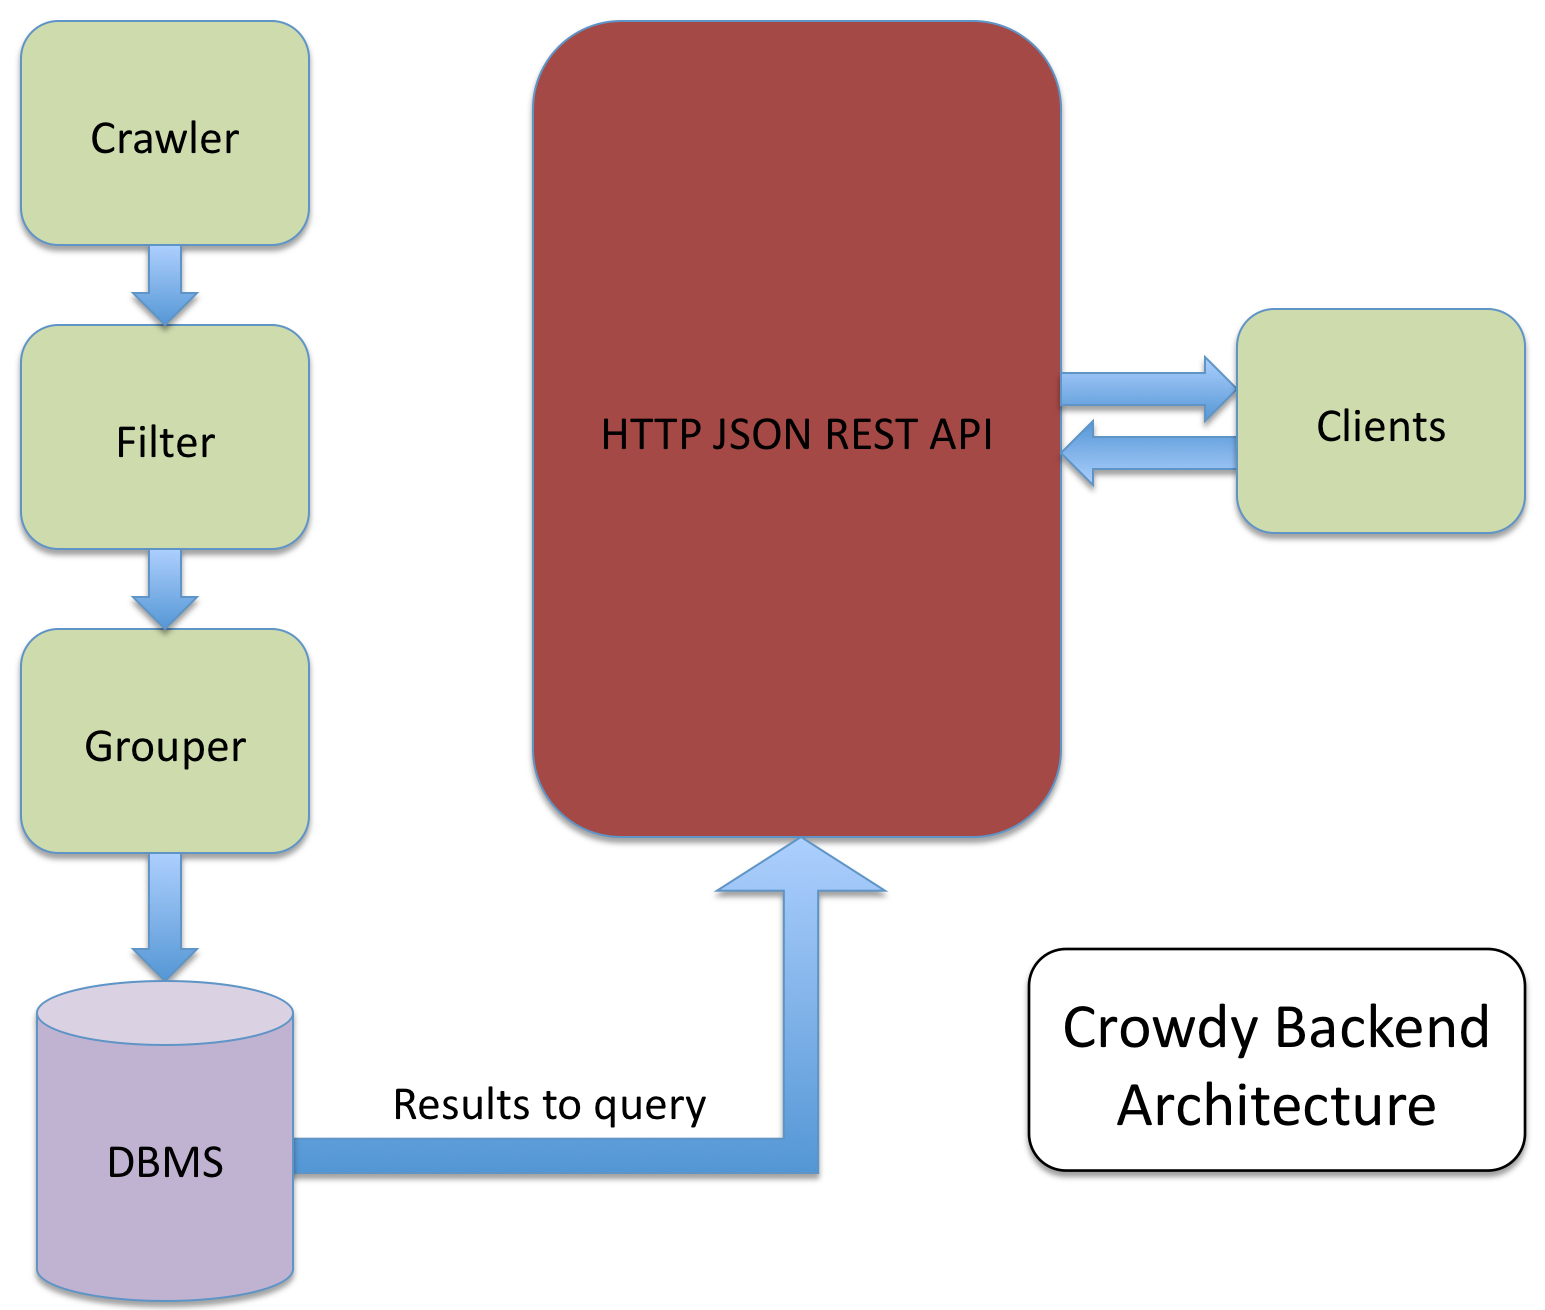
\includegraphics[width=\linewidth]{architecture}
%\caption{CrowdBuzz system architecture. [[REPLACE]]}
%\label{fig:architecture}
%\end{center}
%\end{figure}


\noindent{\textbf {Data Collection Module}}: This is a generic module through
which data is fed into the CrowdBuzz application. In our prototype system, we
collect social messages from the Twitter microblogging service through a mix of
crawling and API calls to the Twitter service. On Twitter, users can post status
updates of 140 characters or less. A status update message posted by user $u_1$
including @$<u_2>$ is considered a message from $u_1$ to $u_2$ 
% (note that users
% other than $u_2$ may view this public message as well)
. The data collection
module collects these messages as tuples $(u_1, u_2, i, t)$, where $i$ is the
message sent from user $u_1$ to $u_2$ at time $t$. The collected tuples are then
passed to the Crowd Discovery module. Note that CrowdBuzz architecture can be
flexibly adapted to other domains supporting social messaging services (e.g.,
Facebook).
% , which has recently adopted a similar user-addressable public messaging
% system within their status updates

\noindent{\textbf {Crowd Discovery Module}}: As user messages are passed to
the Crowd Discovery Module, the CrowdBuzz system analyzes the incoming and
existing messages to find groups of users (what we refer to as \textit{crowds})
who are connected by their communication patterns among each other. Intuitively,
a crowd is a time-sensitive collection of users who have messaged each other
within some recent window of time. We formally define the crowd discovery problem
in the following section as a form of clustering in time-evolving social
networks. The Crowd Discovery Module is designed to maintain up-to-date crowds,
so that social mining analytics can be directly run over the discovered crowds at
occasional intervals (e.g., to identify what the latest buzz is among
communicating groups on Twitter).

\noindent{\textbf {Crowd Evolution Module}}: In addition to providing analytic
services over the current batch of crowds, the CrowdBuzz system also tracks the
evolution of crowds via this third module. For example, as groups of users begin
communicating about an upcoming event (say the Rose Bowl football game), the
evolution module can track the users participating in this crowd and give
insights into the crowd dynamics leading up to and after the event. The Crowd
Evolution module can analyze the discovered crowds from the previous module at
system-specified time intervals to provide varying degrees of evolution
granularity (e.g., for tracking very bursty crowds that grow and disperse over
several hours versus longer-lived crowds that may last for weeks).

\noindent{\textbf {Crowd Visualization and Analytics}}: Finally, the discovered
crowds can be visualized using off-the-shelf visualization tools (e.g., Flare
Prefuse) and mined for concept trends and other important social dynamics. In
this paper, we present some example crowd-based analytics in
Section~\ref{sec:experiments}.

In the rest of the paper, we present the design of the Crowd Discovery module
(Section~\ref{sec:crowd-discovery}) and the Crowd Evolution module
(Section~\ref{sec:crowd-evolution}), as well as the prototype CrowdBuzz
evaluation in Section~\ref{sec:experiments}.

\begin{figure}[!t]
\begin{center}
\includegraphics[width=3.5in]{../../images/www/clusterSize}
\caption{Crowd size distribution.}
\label{fig:count-cluster-size}
\end{center}
\end{figure}

\noindent{\textbf {Crowd size distribution}}: We first consider the size of
crowds discovered. The crowd size distribution for a social network can help
quantify the degree of collaboration within the network. In
Figure~\ref{fig:count-cluster-size} we show the crowd size distribution for
crowds of size greater than or equal to 3 users in our Twitter dataset. We see
that most users on Twitter communicate in small groups, but there are some larger
crowds, with a maximum crowd size of 17. Note that these crowd size distributions
are impacted by the degree of edge damping; varying the edge damping factor $\xi$
can result in large inactive crowds (since old messages can impact crowd
formation), or extremely short-lived crowds (by considering only messages within
the past hour, for example).
\begin{figure}[!t]
\begin{center}
\includegraphics[width=3.5in]{../../images/www/single_multi}
\caption{The figure shows difference between a user-centric and group centric
approach to gather \textit{buzz}.}
\label{fig:single-multi}
\end{center}
\end{figure}




\noindent \textbf{On-Demand Crowd Reporting:} Finally, since the crowd evolution
and analytics tools may only require new crowd information at regular intervals
(e.g., every minute, every hour), we can forgo the cost of constant crowd
maintenance between these intervals through the use of on-demand crowd reporting.


\algsetup{indent=2em}
\newcommand{\DampEdge}{\ensuremath{\mbox{\sc DampEdge}}}
\begin{algorithm}
\caption{$\DampEdge(u, v)$}\label{alg:damp-edge}
\begin{algorithmic}

\IF{$CT - EdgeTime(u, v) > 1$}
\STATE $w(u, v)$ = $w(u, v)- \log(CT - EdgeTime(u, v))\times \xi$ 
\ENDIF
\STATE $EdgeTime(u, v)$ =  $CurrentTime$
\end{algorithmic}
\end{algorithm}

\subsection{Temporal and Spatial Locality on Twitter}


\begin{table}[h]
\centering
\label{table:dataset}
\begin{tabular}{|l|r|}
\hline
\textbf{Messages} & \textbf{Percent of Vertices Affected} \\ \hline
100,000 & 0.2\% \\ \hline
200,000 & 0.5\% \\ \hline
300,000 & 0.6\% \\ \hline
400,000 & 0.9\% \\ \hline
500,000 & 0.9\% \\ \hline
600,000 & 1.7\% \\ \hline
700,000 & 1.5\% \\ \hline
800,000 & 1.6\% \\ \hline

%Interacting user pairs & 500,942 & 5,395\\ \hline
%Directed tweets & 1,243,820 & 7,403\\ \hline
%Status update tweets & 2,972,951 & 17,696\\ \hline
%Average degree & 3.48 & - \\ \hline
\end{tabular}
\caption{Locality Stuff.}
\end{table}

\begin{figure}[!t]
\begin{center}
\includegraphics[width=3.5in]{../../images/sigir/dampRatioAssoc}
\caption{Ratio association value at each time interval for different
damping coefficients.}
\label{fig:damp-ratio-assoc}
\end{center}
\end{figure}

%%%
%%%
%%%
%%%
%%%
\begin{figure}[!t]
\begin{center}
\includegraphics[width=3.5in]{../../images/sigir/dampClusterCount}
\caption{Number of crowds and average crowd sizes at each time interval
for different damping coefficients.}
\label{fig:damp-cluster-count}
\end{center}
\end{figure}